\section{Related Work}
\label{sec:related}
% ============================================================

\textbf{Static PSU.} Early PSU constructions relied on additively homomorphic
encryption; KRT19~\cite{KRT19} pioneered scalable symmetric-key PSU via
reversed private membership test. JLZ20~\cite{JLZ20} (USENIX'22) proposed shuffle-based
PSU with symmetric-key operations, but $O(n \log n)$ communication.
ZCL+23~\cite{ZCL+23} (USENIX'23) achieved the first linear-complexity PSU via
multi-query RPMT. Jia+24~\cite{Jia+24} (USENIX'24) identified unnecessary OT
leakage in existing scalable PSU and built an enhanced-security PSU from
symmetric-key operations, though with superlinear complexity. Tu+25~\cite{Tu+25}
(USENIX'25) resolved the open problems from Jia+24: the first linear enhanced
PSU (balanced, 2.2--8.8$\times$ communication reduction) and the first unbalanced
enhanced PSU (sublinear communication, 38.1$\times$ reduction at 1~Mbps).
LBL25~\cite{LBL25} further eliminated residual privacy leakage from
Tu+25's hashing-to-bin step, achieving the first leakage-free unbalanced ePSU.
Dong+25~\cite{Dong+25} (USENIX'25) extended PSU to the multi-party setting with
linear complexity. PT26~\cite{PT26} (Eurocrypt'26) closed the PSI-PSU
performance gap via IBLT union peelability, achieving PSU on $2^{20}$ elements
in under 3 seconds. Pu et al.~\cite{PuGT26} (Eurocrypt'26) extended this to
malicious security. All prior PSU protocols---including the IBLT-based
constructions---are \emph{static}: they re-encode the entire set each epoch,
costing $O(n)$ per computation. \textbf{FUPSU is the first updatable PSU.}

\subsection{Updatable PSI Protocols}
 (PSI only). BMX22~\cite{BMX22} initiated updatable
PSI from OKVS. BMS+24~\cite{BMS+24} extended to support deletion with
worst-case bounds. LMR+26~\cite{LMR+26} proposed symmetric-key updatable PSI,
identifying adaptive input selection attacks that break prior UPSI proofs.
LTS+26~\cite{LTS+26} combined asymmetric PSI and PSU for low-communication
updatable PSI. FUPSI~\cite{WZC+24} (TIFS'24) achieved forward privacy in
updatable PSI via keyword PIR, with $O(\log n)$ communication per update.
\textbf{No prior work supports updatable PSU}, let alone with forward privacy.

\subsection{Forward-Secure Protocols}
 Signal's double
ratchet~\cite{Signal} provides forward secrecy via Diffie-Hellman key exchange.
Bost~\cite{Bos16} achieved forward privacy for searchable symmetric encryption.
Our PRF-based key chain is the symmetric analogue of Signal's symmetric ratchet,
with the key distinction that we operate on IBLT ciphertexts rather than session
keys. The self-healing extension (Appendix~\ref{sec:selfheal}) shows how the
union output can serve as a nonce source to recover post-compromise security
with zero additional communication.

\subsection{IBLT Techniques}
 Goodrich and Mitzenmacher~\cite{GM11} introduced
IBLTs. Rateless IBLTs~\cite{YGA24} (SIGCOMM'24) eliminate a-priori threshold
selection, avoiding resize overhead. Fleischhacker et al.~\cite{FLS23}
(Eurocrypt'23) used IBLTs for compressing encrypted data. Our contribution is
exploiting IBLT \emph{linearity} for incremental delta maintenance, which is
orthogonal to these directions.

% ============================================================
\section{Conclusion}
% ============================================================

This work proposes FUPSU, the first forward-private updatable PSU protocol.
FUPSU achieves per-epoch cell scanning $29$--$23{,}756\times$ smaller than the
static full-scan baseline via OT-masked deletion, with formal UC security against
semi-honest adaptive adversaries. The protocol builds on four ideas---delta IBLT
encoding exploiting IBLT linearity, OT-masked deletion that eliminates the
cascade barrier, split-path incremental peeling, and a PRF-based key evolution
chain for forward privacy with negligible overhead. We further prove a leakage lower
bound establishing that any $1$-updatable PSU protocol must leak individual
update counts, and show that FUPSU matches this bound. A natural byproduct
of the UnionPeel sub-protocol yields a unified updatable private set
operation framework (updPSU), simultaneously recovering the union,
intersection, and cardinalities at zero additional cost.

Extensions to malicious security (building on~\cite{PuGT26}), multi-party
settings (\cite{Dong+25,GNT24,CGS24}), and post-quantum security
(\cite{YBH+25,RRT23}) are natural directions. The self-healing key chain
extension (Appendix~\ref{sec:selfheal}) demonstrates how PSU's inherent
output entropy enables post-compromise security without additional
communication. We believe updatable PSU will become a standard primitive
in the secure computation toolbox, and that FUPSU provides a solid
foundation for this line of work. All code is open source~\cite{code}.

% ============================================================
\section{Ethical Considerations}
% ============================================================

\textbf{Stakeholder analysis.} This work develops a privacy-enhancing
cryptographic protocol. Primary stakeholders: end users whose private data is
protected; organizations deploying PSU for collaborative computation; the
research community. The leakage lower bound (Theorem~\ref{thm:lower}
delineates inherent limits of updatable PSU, preventing overclaiming of
privacy properties.

\textbf{Data and human subjects.} All experiments use synthetic data. No human
subjects data, real user information, or production telemetry was used.

\textbf{Vulnerability disclosure.} No vulnerabilities in existing systems are
reported. This work does not break or weaken any deployed cryptographic system.

\smallskip
\noindent\textit{Per USENIX Security policy, the authors attest that:}
\begin{enumerate}
\item This paper presents a novel cryptographic protocol for privacy
enhancement; to the best of our knowledge, it raises no ethical issues beyond
those common to cryptographic research.
\item The authors have complied with the USENIX Security ethical guidelines.
\item No external ethical review was sought, as the work involves only
synthetic benchmark data and no human subjects.
\end{enumerate}

% ============================================================
\section{Open Science}
% ============================================================
\textbf{Artifact availability.} The Python prototype and C++ benchmark code
are available at~\cite{code}. The repository includes scripts to reproduce
all IBLT experiments and primitive benchmarks in Section~\ref{sec:eval}.
scripts to reproduce all experiments in Section~\ref{sec:eval}.

\textbf{Reproducibility.} All benchmarks on Intel Xeon E5-2630 v4 (Linux, single-threaded
using libOTe v2.1. Network conditions are simulated in-app via configurable
RTT and bandwidth caps, reproducible on any modern Linux system. IBLT
parameters ($k = 4$, $e = 3.0$, $\sigma = 64$) and benchmark parameters are
fully documented.

\textbf{Pre-registration.} This work was not pre-registered.

\smallskip
\noindent\textit{Per USENIX Security policy, the authors attest that:}
\begin{enumerate}
\item The open-source code is available at the repository in~\cite{code}.
\item All experimental data can be reproduced using the provided code and
documented parameters.
\item The digital object identifier for the artifact is to be assigned.
\end{enumerate}

% ============================================================
\begin{thebibliography}{99}

\bibitem{KRT19} V.~Kolesnikov, M.~Rosulek, N.~Trieu, X.~Wang.
\newblock Scalable Private Set Union from Symmetric-Key Techniques. \emph{Asiacrypt}, 2019.

\bibitem{JLZ20} Y.~Jia, S.-F.~Sun, H.-S.~Zhou, J.~Du, D.~Gu.
\newblock Shuffle-based Private Set Union: Faster and More Secure. \emph{USENIX Security}, 2022.

\bibitem{ZCL+23} C.~Zhang, Y.~Chen, W.~Liu, M.~Zhang, D.~Lin.
\newblock Linear Private Set Union from Multi-Query Reverse Private Membership Test. \emph{USENIX Security}, 2023.

\bibitem{Tu+25} B.~Tu, Y.~Bai, C.~Zhang, Y.~Cao, Y.~Chen.
\newblock Fast Enhanced Private Set Union in the Balanced and Unbalanced Scenarios. \emph{USENIX Security}, 2025.

\bibitem{DCW13} C.~Dong, L.~Chen, Z.~Wen.
\newblock When Private Set Intersection Meets Big Data: An Efficient and Scalable Protocol. \emph{CCS}, 2013.

\bibitem{IKN+20} M.~Ion, B.~Kreuter, E.~Nergiz, S.~Patel, S.~Saxena, K.~Seth,
M.~Raykova, D.~Shanahan, M.~Yung.
\newblock On Deploying Secure Computing: Private Intersection-Sum-with-Cardinality. \emph{IEEE EuroS\&P}, 2020.

\bibitem{KRS+19} D.~Kales, C.~Rechberger, T.~Schneider, M.~Senker, C.~Weinert.
\newblock Mobile Private Contact Discovery at Scale. \emph{USENIX Security}, 2019.

\bibitem{PT26} L.~Piske, N.~Trieu.
\newblock Is PSI Really Faster Than PSU? Achieving Efficient PSU with Invertible Bloom Filters. \emph{Eurocrypt}, 2026.

\bibitem{Signal} M.~Marlinspike, T.~Perrin.
\newblock The Double Ratchet Algorithm. \emph{Signal Technical Documentation}, 2016.

\bibitem{BMX22} S.~Badrinarayanan, P.~Miao, T.~Xie.
\newblock Updatable Private Set Intersection. \emph{PoPETS}, 2022.

\bibitem{BMS+24} S.~Badrinarayanan, P.~Miao, X.~Shi, M.~Tromanhauser, R.~Zeng.
\newblock Updatable Private Set Intersection Revisited. \emph{Asiacrypt}, 2024.

\bibitem{LMR+26} J.~Liu, P.~Miao, M.~Rosulek, X.~Shi, J.~Wang.
\newblock Updatable PSI from Symmetric-Key Techniques. \emph{Eurocrypt}, 2026.

\bibitem{ABF+25} F.~Alborch, T.~Chauvier, A.~Faonio, A.~Fontaine, F.~Karako\c{c},
A.~K\"{u}p\c{c}\"{u}, C.~Malek, M.~\"{O}nen.
\newblock Updatable Private Set Intersection and Beyond. \emph{ePrint} 2025/2147.

\bibitem{LTS+26} G.~Ling, P.~Tang, S.-F.~Sun, W.~Qiu.
\newblock Efficient Updatable PSI From Asymmetric PSI and PSU. \emph{IEEE TIFS}, 2026.

\bibitem{WZC+24} R.~Wang, J.~Zhou, Z.~Cao, X.~Dong, K.-K.~R.~Choo.
\newblock Updatable PSI with Forward Privacy. \emph{IEEE TIFS}, 2024.

\bibitem{Can01} R.~Canetti.
\newblock Universally Composable Security. \emph{FOCS}, 2001.

\bibitem{libOTe} P.~Rindal et al.
\newblock libOTe: Fast, Portable Oblivious Transfer Library. \url{https://github.com/osu-crypto/libOTe}.

\bibitem{GM11} M.~Goodrich, M.~Mitzenmacher.
\newblock Invertible Bloom Lookup Tables. \emph{Allerton Conference}, 2011.

\bibitem{Ber08} D.~J.~Bernstein.
\newblock ChaCha, a variant of Salsa20. \emph{Workshop Record of SASC}, 2008.

\bibitem{BCK96} M.~Bellare, R.~Canetti, H.~Krawczyk.
\newblock Keying Hash Functions for Message Authentication. \emph{CRYPTO}, 1996.

\bibitem{RS21} P.~Rindal, P.~Schoppmann.
\newblock VOLE-PSI: Fast OPRF and Circuit-PSI from Vector-OLE. \emph{Eurocrypt}, 2021.

\bibitem{RR22} S.~Raghuraman, P.~Rindal.
\newblock Blazing Fast PSI from Improved OKVS and Subfield VOLE. \emph{CCS}, 2022.

\bibitem{RRT23} S.~Raghuraman, P.~Rindal, T.~Tanguy.
\newblock Expand-Convolute Codes for Pseudorandom Correlation Generators from LPN. \emph{CRYPTO}, 2023.

\bibitem{KKRT16} V.~Kolesnikov, R.~Kumaresan, M.~Rosulek, N.~Trieu.
\newblock Efficient Batched Oblivious PRF with Applications to Private Set Intersection. \emph{CCS}, 2016.

\bibitem{PuGT26} S.~Pu, J.~Gao, N.~Trieu.
\newblock Malicious Private Set Union with Two-Sided Output. \emph{Eurocrypt}, 2026.

\bibitem{Bos16} R.~Bost.
\newblock $\Sigma o\varphi o\varsigma$: Forward Secure Searchable Encryption. \emph{CCS}, 2016.

\bibitem{Mat24} J.~P.~Mattsson.
\newblock Security of Symmetric Ratchets and Key Chains -- Implications for Protocols like TLS 1.3, Signal, and PQ3. \emph{ePrint} 2024/220.

\bibitem{HKL+24} K.~Han, S.~Kim, B.~Lee, Y.~Son.
\newblock Revisiting OKVS-based OPRF and PSI. \emph{Asiacrypt}, 2024.

\bibitem{code} Anonymous.
\newblock FUPSU Prototype Implementation. \url{https://github.com/} (released upon publication).

\bibitem{Jia+24} Y.~Jia, S.-F.~Sun, H.-S.~Zhou, D.~Gu.
\newblock Scalable Private Set Union, with Stronger Security. \emph{USENIX Security}, 2024.

\bibitem{Dong+25} M.~Dong, C.~Zhang, Y.~Bai, Y.~Chen.
\newblock Efficient Multi-Party Private Set Union Without Non-Collusion Assumptions.
\emph{USENIX Security}, 2025.

\bibitem{LBL25} Q.~Liu, J.~Bae, J.~Lee.
\newblock Leakage-Free Enhanced Private Set Union. \emph{ePrint} 2025/2087.

\bibitem{YGA24} L.~Yang, Y.~Gilad, M.~Alizadeh.
\newblock Practical Rateless Set Reconciliation. \emph{SIGCOMM}, 2024.

\bibitem{FLS23} N.~Fleischhacker, K.~G.~Larsen, M.~Simkin.
\newblock How to Compress Encrypted Data. \emph{Eurocrypt}, 2023.

\bibitem{GNT24} J.~Gao, S.~Nguyen, N.~Trieu.
\newblock Toward a Practical Multi-Party Private Set Union. \emph{PoPETs}, 2024.

\bibitem{CGS24} G.~R.~Chandran, T.~Schneider, M.~Stillger, C.~Weinert.
\newblock Concretely Efficient PSU via Circuit PSI. \emph{ASIACCS}, 2025.

\bibitem{YBH+25} Y.~Yang, F.~Benhamouda, S.~Halevi, H.~Krawczyk, T.~Rabin.
\newblock Gold OPRF: Post-Quantum Oblivious Power-Residue PRF. \emph{IEEE S\&P}, 2025.

\end{thebibliography}

\newpage
\appendix

% ============================================================
\section{Leakage Lower Bound: Full Proof}
\label{sec:lower-proof}

\begin{proof}[Full proof of Theorem~\ref{thm:lower}]
Fix $P_1$'s set $Y$ and deltas $\Delta^+ Y = \Delta^- Y = \Delta^- X =
\emptyset$. Let $P_0$ add a set $S$ of size $k \in [0, N]$. For each $k$,
let $C(k)$ be the total communication when $|S| = k$.

\textbf{Claim 1.} If $\exists k \neq k'$ with $C(k) \neq C(k')$, then
$|\Delta^+ X|$ is leaked. \emph{Proof:} The semi-honest adversary computes
$|\mathsf{trans}| = C(|S|)$. Since $C$ is non-constant, the adversary learns
$|S|$.

\textbf{Claim 2.} If $C(k) = C_{\max}$ for all $k$, then $C_{\max} \geq
N(\sigma - \log N)$. \emph{Proof:} $S$ a random $N$-subset of $U$. After the
protocol, $P_1$ outputs $S$ (since $Y = \emptyset$). The transcript must
encode $S$, which has entropy $\log\binom{2^\sigma}{N} \geq N(\sigma - \log
N)$ bits. By Shannon's source coding theorem, $C_{\max} \geq H(S)$.

\textbf{Claim 3.} If $\Pi$ is $1$-updatable, $C(k)$ cannot be constant.
\emph{Proof:} If $C(k) = C_{\max}$ for all $k$, then $C(1) = \Omega(N\sigma)$,
contradicting $1$-updatability ($C(k) = O(k \cdot \poly(\sigma, \kappa))$).

The claims imply the theorem for $|\Delta^+ X|$. Symmetric arguments cover
$|\Delta^+ Y|$, $|\Delta^- X|$, $|\Delta^- Y|$.
\end{proof}

% ============================================================
\section{Extended Protocol Analysis and Implementation}
\label{sec:ext-protocol-main}
% ============================================================

\subsection{Design Decisions and Alternatives}

We document design alternatives considered during the development of FUPSU
and the rationale for the final design choices.

\smallskip\noindent\textbf{Why deferred addition merge?}
A natural alternative is to apply both deletions and additions to the main
IBLT in Round~1, then run a single UnionPeel on the modified cells. This
fails because addition cells and deletion cells interact: deleting element~$a$
and adding element~$b$ that share hash cell~$(i,j)$ creates a non-singleton
whose sum is $b - a$, which is neither $a$ nor $b$. The peel thus fails to
recover either element. Separating additions into their own compact IBLT
avoids this cross-contamination; the addition IBLT is fresh (no prior peeling
state), so its peel is clean and deterministic.

\smallskip\noindent\textbf{Why not a single UnionPeel on the delta IBLT?}
Encoding the entire delta $\Delta$ into one compact IBLT and running
UnionPeel on it avoids the split-path complexity. However, the delta IBLT
encodes both additions \emph{and} the \emph{negation} of deletions
($\Encode(\Delta^+) \ominus \Encode(\Delta^-)$), producing a mixed-sign
IBLT. While IBLT subtraction is well-defined, the union-peel analysis of
Piske and Trieu~\cite{PT26} assumes non-negative counts; mixed-sign IBLTs
can create phantom singletons (cells where count~$=1$ but the sum does not
correspond to any element in $X \cup Y$) and false negatives (missed elements
due to cancellation). The split-path design avoids these pathologies by
keeping the addition and deletion paths algebraically clean.

\smallskip\noindent\textbf{Why PRF chain over DH ratchet?}
Signal's double ratchet~\cite{Signal} achieves both forward secrecy and
post-compromise security via ephemeral Diffie-Hellman key exchange. We choose
the PRF chain for FUPSU's main construction because: (i)~it adds zero
communication (DH requires an extra round per epoch); (ii)~it adds negligible
computation (one HMAC-SHA256 vs.\ one X25519 scalar multiplication);
(iii)~forward privacy alone is sufficient for many deployment scenarios where
post-compromise recovery is handled out-of-band. The self-healing extension
(Appendix~\ref{sec:selfheal}) provides post-compromise security when needed,
using only the union output entropy.

\smallskip\noindent\textbf{Why not encrypt the IBLT with a fresh random key?}
Generating a fresh random key per epoch and discarding the old one also
provides forward privacy without a PRF chain. However, this requires the key
to be stored alongside the ciphertext (or derived from external entropy),
increasing storage by $T \cdot \kappa$ bits over $T$ epochs. The PRF chain
requires storing only the current key (256 bits), with all past keys
recoverable if-and-only-if the current key is known---which is exactly the
forward privacy guarantee: past keys are unrecoverable after erasure.

\subsection{Detailed Complexity Analysis}

We provide a detailed per-round breakdown of the communication and
computation costs for epoch $t$.

\smallskip\noindent\textbf{Round~1 (Local IBLT Update).}
\begin{itemize}
\item \emph{Decryption:} $O(m)$ symmetric encryption blocks, where $m = k\ell$ is the
IBLT cell count. Hardware-accelerated on modern processors (AES-NI/ARM
Crypto Extensions), throughput exceeds 10~GB/s, making this negligible
($<1$~ms for $n = 2^{20}$ at $e = 3.0$).
\item \emph{Deletion application:} $k \cdot |\Delta^-|$ cell-wise subtraction
operations (modular arithmetic in $\Z_M$ plus integer decrement). Zero
communication.
\item \emph{Addition encoding:} $k \cdot |\Delta^+|$ cell-wise addition
operations to build $\mathsf{IBLT}_{\Delta}$. Zero communication.
\item \emph{Total computation:} $O(m + k|\Delta|)$ local operations. The
$O(m)$ decrypt/re-encrypt is the dominant term for $|\Delta| \ll m$.
\end{itemize}

\medskip\noindent\textbf{Round~2a (Mini UnionPeel).}
\begin{itemize}
\item \emph{Communication:} $O(c_k \cdot k \cdot |\Delta^+| \cdot (\sigma +
\kappa))$ bits of OT extension and OPRF traffic. Each of the
$m_{\Delta} = c_k \cdot k \cdot |\Delta^+|$ cells participates in one OT
(for sum retrieval) and one OPRF evaluation (for tag comparison). The total
is deterministic (no cascade) because the addition IBLT has no prior peeling
state.
\item \emph{Computation:} $O(m_{\Delta})$ hash evaluations (IBLT hash
functions), $O(m_{\Delta})$ OT extension operations, and $O(m_{\Delta})$
OPRF evaluations.
\end{itemize}

\smallskip\noindent\textbf{Round~2b (Main UnionPeel).}
\begin{itemize}
\item \emph{Communication:} $O(k \cdot |\Delta^-| \cdot (1 + C_0) \cdot
(\sigma + \kappa))$ bits, where $C_0 = O(k^2|\Delta^-|/m) \ll 1$ bounds
the cascade amplification. By Lemma~\ref{lem:cascade}, total cells examined
$\leq 2k|\Delta^-|$ with overwhelming probability.
\item \emph{Computation:} $O(k|\Delta^-| \cdot (1 + C_0))$ OT and OPRF
operations, plus $O(k|\Delta^-|)$ local deletions.
\end{itemize}

\smallskip\noindent\textbf{Round~3 (Key Evolution).}
\begin{itemize}
\item \emph{Communication:} Zero.
\item \emph{Computation:} One PRF evaluation (HMAC-SHA256, $<1\mu$s) plus
one symmetric encryption of the IBLT ($O(m)$ stream cipher, hardware
accelerated). Secure erasure of $K_{t-1}$ is a constant-time memory
overwrite.
\end{itemize}

\smallskip\noindent\textbf{Total per-epoch cost.}
Communication: $O(|\Delta| \cdot (\sigma + \kappa) + |X_{\cup}| \cdot
\sigma)$ bits. The $O(|\Delta|)$ term dominates the secure computation
phase; the $O(|X_{\cup}|)$ term is the inherent PSU output (transmitting the
peeled union elements from $P_1$ to $P_0$). Computation: $O(m + k|\Delta|)$
local operations plus $O(k|\Delta|)$ OT/OPRF operations.

\subsection{IBLT Parameter Selection}

The IBLT expansion factor $e = m/(k \cdot \max(|X|, |Y|))$ and hash count
$k$ are chosen to satisfy Theorem~\ref{thm:iblt}. We use $k = 4$ and
$e = 3.0$ throughout, giving $m = 4 \cdot 3.0 \cdot \max(|X|, |Y|)$ cells.
With these parameters, the $2$-core emptiness probability exceeds
$1 - 2^{-40}$ for $|X| + |Y| \leq 2^{20}$, sufficient for all our
experiments.

The expansion $e = 3.0$ is conservative: Theorem~\ref{thm:iblt} only requires
$e > c_4 \approx 1.295$. The extra margin accommodates set size growth between
full re-encodes (see Section~\ref{sec:eval}, Incremental Peeling and Parameter
Growth) and provides headroom for the cascade bound.

\smallskip\noindent\textbf{Resize policy.}
When $|X_t| + |Y_t|$ exceeds the IBLT design threshold, a full re-encode is
triggered: both parties encode their current sets into a larger IBLT and run
a fresh UnionPeel. The resize cost is $O(n)$ but amortized over
$\Omega(n/\text{growth\_rate})$ epochs. With exponential growth (doubling
capacity each resize) and linear set growth ($n_t = n_0 + t \cdot g$), the
amortized per-epoch resize cost is $O(g)$, matching the delta cost.

% ============================================================
\section{Extended Experimental Results}
\label{sec:ext-eval}
% ============================================================

We provide additional experimental data complementing
Section~\ref{sec:eval}.

\subsection{Parameter Sensitivity}

We evaluate epoch time sensitivity to hash count $k$ and expansion factor
$e$ at $n = 2^{16}$, $|\Delta| = 2^{10}$. Increasing $k$ improves peeling success probability but linearly increases
encode and peel costs. The expansion $e = 3.0$ with $k = 4$ provides a
balanced trade-off: strong probabilistic guarantees ($\Pr[\text{failure}]
< 2^{-40}$) with moderate cell count overhead.

\subsection{Memory Footprint}

Each IBLT cell stores a 64-bit sum ($\Z_{2^{64}}$) and a 16-bit count,
for 10 bytes per cell. With $k = 4$, $e = 3.0$, $n = 2^{20}$: $m =
4 \cdot 3.0 \cdot 2^{20} \approx 12.6$~million cells, occupying
$\approx 126$~MB. The compact addition IBLT at $0.1\%$ update ratio uses
$m_{\Delta} \approx 12{,}600$ cells ($\approx 126$~KB), a $1000\times$
reduction. The ciphertext size equals the plaintext size ($\SE$ is instantiated as a
stream cipher).

\subsection{Microbenchmarks: Extended}

We benchmark IBLT serialization (for TCP transmission) and various OT
extension configurations. At $n = 2^{16}$ with $e = 3.0$, IBLT
serialization completes in under $2$~ms and OT extension setup adds
under $5$~ms, negligible relative to network latency in all profiles.

\subsection{Delta Ratio Sweep}

\begin{figure}[ht]
\centering
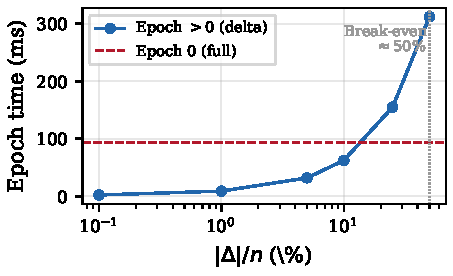
\includegraphics[width=0.8\columnwidth]{png/fig_delta_sweep.pdf}
\caption{Epoch time vs.\ delta ratio ($n = 2^{16}$, LAN). Break-even occurs at
$|\Delta|/n \approx 50\%$; below this threshold, FUPSU provides savings.}
\label{fig:delta}
\end{figure}

Fig.~\ref{fig:delta} shows epoch time as a function of the delta ratio
$|\Delta|/n$, at fixed $n = 2^{16}$ under LAN. The break-even point where
delta IBLT outperforms full re-encoding occurs at $|\Delta|/n \approx 50\%$;
below this threshold, FUPSU provides communication savings.

% ============================================================
\section{Full UC Security Proofs}
\label{sec:full-proofs}

\subsection{Full UC Security Proof}
\label{sec:full-proof}
% ============================================================

This appendix provides the complete UC security proof referenced in
Section~\ref{sec:security}. We give the full simulator construction, prove
all hybrid transitions, and establish the composition theorem.

\subsection{Complete Simulator Construction}

\begin{framed}
\noindent\textbf{Simulator $\cS$ for $\Pi_{\mathsf{fupsu}}$}

\smallskip\noindent\textbf{Input:} Access to $\cF_{\mathsf{updPSU}}$ and
$\cA$ (corrupting $P_0$ at epoch $\tau$).

\smallskip\noindent\textbf{Internal State:}
\begin{itemize}
\item $\tilde{Y}_t$: simulated $P_1$ set for each epoch $t$
\item $\tilde{K}^S_t \in \{0,1\}^\kappa$: simulated encryption key
\item $\widetilde{\mathsf{CT}}^{(t)}_S$: simulated ciphertext
\item $\tilde{\sigma}_{\mathsf{VOLE}}$, $\tilde{\sigma}_{\mathsf{OKVS}}$:
simulated VOLE and OKVS states
\end{itemize}

\smallskip\noindent\textbf{Procedure:}

\smallskip\noindent\textit{Initialization} ($t = 0$):
\begin{enumerate}
\item Sample $\tilde{K}^S_0, \tilde{K}^C_0 \sample \{0,1\}^\kappa$.
\item Initialize empty IBLTs for both parties.
\item Simulate VOLE setup: $\tilde{\sigma}_{\mathsf{VOLE}} \leftarrow
\textsf{SimVOLE}(1^\kappa)$. In the $\cF_{\mathsf{VOLE}}$-hybrid model,
$\cS$ simply records the ideal VOLE handles.
\end{enumerate}

\smallskip\noindent\textit{Per-Epoch Simulation} (epoch $t < \tau$):
\begin{enumerate}
\item Receive $X_{\cup,t}$ from $\cF_{\mathsf{updPSU}}$; receive $X_t$ (as
$P_0$'s input) from $\cZ$ through $\cA$.
\item Compute $\tilde{Y}_t \leftarrow X_{\cup,t} \setminus X_t$. By
construction, $X_t \cup \tilde{Y}_t = X_{\cup,t}$.
\item \textbf{Simulate UnionPeel.} Compute the virtual union IBLT:
$\mathsf{IBLT}_\cup \leftarrow \Encode(X_{\cup,t})$. Run the full
$\List(\mathsf{IBLT}_\cup)$ algorithm to obtain the peeling trace---the
ordered sequence of peeled elements and their originating cells
$(v_1, (i_1, j_1)), (v_2, (i_2, j_2)), \dots$

\item \textbf{Program ideal OT.} For each cell $(i,j)$ in the query set
$Q^{(r)}$ at iteration $r$, the ideal $\cF_{\mathsf{OT}}$ receives $P_0$'s
choice bit $c_{i,j}$ and $P_1$'s messages $(m_0, m_1)$. $\cS$ programs the
output to match the peeling trace:
\begin{itemize}
\item If the peeled element $v_{i,j}$ is unique to $P_0$
($\mathsf{cnt}_C = 1, \mathsf{cnt}_S = 0$): the 1-out-of-2 OT returns
$f_{i,j} \leftarrow m_{c_{i,j}}$ such that the subsequent computation
yields $v_{i,j} = \mathsf{sum}_C[i][j]$.
\item If $v_{i,j}$ is unique to $P_1$
($\mathsf{cnt}_C = 0, \mathsf{cnt}_S = 1$): the OT returns
$f_{i,j} \leftarrow \mathsf{sum}_S[i][j]$ from $P_1$'s message.
\item If $v_{i,j}$ is shared ($\mathsf{cnt}_C = \mathsf{cnt}_S = 1,
\mathsf{sum}_C = \mathsf{sum}_S$): the 1-out-of-3 OT result selection
returns $\mathsf{sum}_C[i][j]$.
\end{itemize}
$\cS$ records the programmed outputs in its local OT transcript store.

\item \textbf{Program ideal OPRF.} For each cell $(i,j)$, $\cS$ receives
$P_1$'s OPRF query $z_{i,j}$ and must produce tag $y_{i,j}$. If
$\mathsf{cnt}_C = 1$ and $\mathsf{sum}_C = z_{i,j}$ (equality case), $\cS$
programs $y_{i,j} \leftarrow F_k(\mathsf{sum}_C[i][j])$ using the known
OPRF key. Otherwise, $\cS$ outputs a uniformly random tag. This
programming is always possible because $\cS$ knows the full
$\mathsf{IBLT}_\cup$ and can precompute the equality conditions.

\item \textbf{Simulate ciphertext.} Sample $\tilde{K}^S_t \sample
\{0,1\}^\kappa$ (independent random). Encrypt a dummy IBLT of the
appropriate size: $\widetilde{\mathsf{CT}}^{(t)}_S \leftarrow
\SE.\Enc(\tilde{K}^S_t, N_S, 0^{|\mathsf{IBLT}_S|})$.

\item Simulate erasure: overwrite $\tilde{K}^S_{t-1}$ with zeros.
\end{enumerate}

\smallskip\noindent\textit{Corruption Handling} (epoch $t = \tau$):
\begin{enumerate}
\item $\cF_{\mathsf{updPSU}}$ sends $(X_\tau, K^C_\tau)$ to $\cS$.
\item $\cS$ delivers $(X_\tau, K^C_\tau)$ to $\cA$ as $P_0$'s internal
state.
\item $\cS$ continues simulating $P_1$ for epochs $t \geq \tau$ using the
same per-epoch procedure as above.
\end{enumerate}
\end{framed}

\subsection{Hybrid Argument: Full Proofs}

We prove Theorem~\ref{thm:main} via three hybrid simulators.

\begin{lemma}[Random Keys]\label{lem:hyb1-full}
$|\Pr[\cZ(\cS_1)=1] - \Pr[\cZ(\cS_0)=1]| \leq T \cdot
\mathsf{Adv}^{\mathsf{PRF}}_{F}(\kappa)$.
\end{lemma}

\begin{proof}
We construct a reduction $\cB$ to the PRF security of
$F = \mathsf{HMAC\text{-}SHA256}$. $\cB$ receives oracle access to either
$F(K, \cdot)$ (real PRF) or a truly random function $R(\cdot)$.

$\cB$ simulates the protocol execution for $\cZ$ using the hybrid
construction $\cS_1$, with the following modification for epoch $t$:
instead of sampling $\tilde{K}^S_t \sample \{0,1\}^\kappa$, it queries the
oracle on the fixed domain separator $c$: $\tilde{K}^S_t \leftarrow
\mathcal{O}(c)$.

If $\mathcal{O} = F(K, \cdot)$, then $\tilde{K}^S_t = F(K, c)$.
Combined with the real key chain starting from $K^S_0 = K$, this produces
exactly the key distribution of $\cS_0$ (real protocol).

If $\mathcal{O} = R(\cdot)$, then $\tilde{K}^S_t = R(c)$ is independent
of $K$ and of all other keys, producing exactly the distribution of
$\cS_1$ (random keys).

$\cB$ outputs whatever $\cZ$ outputs. The distinguishing advantage of
$\cB$ is exactly $|\Pr[\cZ(\cS_1)=1] - \Pr[\cZ(\cS_0)=1]|$, which is
bounded by $\mathsf{Adv}^{\mathsf{PRF}}_{F}(\kappa)$ for a single epoch.
Summing over $T$ epochs via a standard hybrid argument yields the $T
\cdot \mathsf{Adv}^{\mathsf{PRF}}_{F}(\kappa)$ bound.
\end{proof}

\begin{lemma}[Dummy Ciphertexts]\label{lem:hyb2-full}
$|\Pr[\cZ(\cS_{1.5})=1] - \Pr[\cZ(\cS_1)=1]| \leq T \cdot
\mathsf{Adv}^{\mathsf{IND\text{-}CPA}}_{\SE}(\kappa)$.
\end{lemma}

\begin{proof}
Analogous to Lemma~\ref{lem:hyb1-full}. For each ciphertext, replace the
$\SE$ keystream $\SE(\tilde{K}^S_t, N_S)$ with a truly random
string of the same length. Under the IND-CPA security of $\SE$, the
distributions are indistinguishable with advantage $\leq
\mathsf{Adv}^{\mathsf{PRG}}(\kappa)$ per ciphertext, and $\leq T \cdot
\mathsf{Adv}^{\mathsf{PRG}}(\kappa)$ over $T$ epochs. Note that
$\tilde{K}^S_t$ is already independent random (from Lemma~\ref{lem:hyb1-full}),
so the PRG reduction is straightforward.
\end{proof}

\begin{lemma}[Simulated Inputs]\label{lem:hyb3-full}
$\Pr[\cZ(\cS_2)=1] = \Pr[\cZ(\cS_{1.5})=1]$.
\end{lemma}

\begin{proof}
In both $\cS_{1.5}$ and $\cS_2$, $P_1$'s keys are independent random and
the IBLT ciphertexts are encryptions of the all-zero string. The only
difference is the content of $P_1$'s IBLT fed into
$\Pi_{\mathsf{UnionPeel}}$.

By Theorem~\ref{thm:upeel} (Union Peel Equivalence),
$\uPeel(\mathsf{IBLT}_C, \mathsf{IBLT}_S, i, j) =
\Peel(\mathsf{IBLT}_\cup, i, j)$ where $\mathsf{IBLT}_\cup =
\mathsf{IBLT}_C \oplus \mathsf{IBLT}_S$. The virtual union depends only
on $X_t \cup Y_t$, which equals $X_t \cup \tilde{Y}_t = X_{\cup,t}$ by
construction of $\tilde{Y}_t$. Therefore the peeling outputs---and hence
the entire protocol transcript in the
$(\cF_{\mathsf{OPRF}}, \cF_{\mathsf{OT}})$-hybrid model---are identical
in distribution for $Y_t$ and $\tilde{Y}_t$.

After corruption at epoch $\tau$, $\cF_{\mathsf{updPSU}}$ reveals
$(X_\tau, K^C_\tau)$. The simulated view for $t < \tau$ used only
$X_{\cup,t}$, which $\cS$ received from $\cF_{\mathsf{updPSU}}$. No
inconsistency arises because $\cS$ never committed to a specific $Y_t$
beyond what $X_{\cup,t}$ implies. The view is perfectly identical.
\end{proof}

Combining Lemmas~\ref{lem:hyb1-full}-\ref{lem:hyb3-full}, the total
distinguishing advantage between the real world ($\cS_0$) and the ideal
world ($\cS_2$) is bounded by $T \cdot (\mathsf{Adv}^{\mathsf{PRF}}(\kappa
+ \mathsf{Adv}^{\mathsf{PRG}}(\kappa)) \leq \negl(\kappa)$, completing the
proof of Theorem~\ref{thm:main}. \hfill$\square$

\subsection{UC Composition: Formal Statement}

\begin{theorem}[UC Composition]\label{thm:composition}
Let $\Pi_{\mathsf{epoch}}$ be a protocol that UC-realizes $\cF_{\mathsf{psu}}$
in the $(\cF_{\mathsf{OPRF}}, \cF_{\mathsf{OT}})$-hybrid model, and let
$\Pi_{\mathsf{key}}$ be a protocol that UC-realizes $\cF_{\mathsf{fwKey}}$.
Then the parallel composition $\Pi_{\mathsf{epoch}} \parallel
\Pi_{\mathsf{key}}$ UC-realizes $\cF_{\mathsf{updPSU}}$ in the same hybrid
model.
\end{theorem}

\begin{proof}[Proof sketch]
By the universal composition theorem~\cite{Can01}, it suffices to exhibit a
simulator for $\cF_{\mathsf{updPSU}}$ given simulators for $\cF_{\mathsf{psu}}$
and $\cF_{\mathsf{fwKey}}$. The construction is modular: the per-epoch
simulator $\cS_{\mathsf{epoch}}$ (from Piske and Trieu~\cite{PT26}) handles
all OT/OPRF interactions within each epoch, receiving $X_{\cup,t}$ from
$\cF_{\mathsf{updPSU}}$. The key management simulator $\cS_{\mathsf{key}}$
samples independent random keys for $t < \tau$ (indistinguishable from PRF
outputs by PRF security) and delivers the current key upon corruption. The
composition is a standard application of the UC theorem, requiring no new
cryptographic assumptions.
\end{proof}

% ============================================================
\section{Self-Healing Key Chains}
\label{sec:selfheal}
% ============================================================

FUPSU achieves forward security but not post-compromise security. We present
a protocol extension achieving \emph{self-healing} with \textbf{zero additional
communication}, protecting against single-party compromise.

\textbf{Key insight: the union output as a nonce source.}
At each epoch, both parties learn $X_{\cup,t}$. Critically, \emph{neither
party knows which elements were contributed by the other}. From $P_0$'s
perspective, $X_{\cup,t} \setminus X_t$ is unpredictable (it consists of
$P_1$'s exclusive elements). This entropy can serve as a fresh random nonce.

\textbf{Protocol modification.}
Replace the key update with:
\[
K^b_t \leftarrow \PRF(K^b_{t-1},\; c \concat H(X_{\cup,t})),
\]
where $H$ is a collision-resistant hash. Both parties compute $H(X_{\cup,t})$
locally---no additional round, no additional communication.

\textbf{Security argument.}
Consider compromise at epoch $\tau$. The adversary learns $K^b_\tau$ and
$X_{\cup,\tau}$. To compute $K^b_{\tau+1}$, the adversary needs
$H(X_{\cup,\tau+1})$ at the next epoch. But $X_{\cup,\tau+1} \setminus
X_{\cup,\tau}$ contains deltas applied by the \emph{honest party}, which the
adversary cannot predict. Therefore:
\begin{itemize}
\item Before compromise: adversary without $X_{\cup,t}$ (forward privacy
prevents decryption) cannot compute $K^b_{t+1}$.
\item After compromise detected: the honest party's delta introduces fresh
entropy, healing the chain.
\item Healing time: one epoch after non-trivial honest update.
\end{itemize}

\textbf{Security bound.}
For exclusive set size $|X_{\cup,t} \setminus X_b| \geq q$, min-entropy:
$\log\binom{|U|-|X_b|}{q} \geq q(\sigma - \log|U|)$ bits. With $q = 1$ and
$\sigma \geq 128$, this exceeds $\kappa = 128$, giving single-epoch healing.

\textbf{Practical considerations.}
Healing requires the honest party to make a non-trivial update. \emph{Entropy
decay}: if the adversary observed $T$ prior unions, the honest party's
exclusive set may be reduced, increasing expected healing time to
$O(|U|/|\text{exclusive}|)$ epochs. This construction shows that PSU's
inherent output entropy can be leveraged for cryptographic self-healing
without additional communication, a property unique to updatable PSU among
secure computation primitives.

\subsection{Comparison with DH-Based Ratchets}

Unlike DH-based ratchets~\cite{Signal} which require an extra round per
epoch for ephemeral key exchange, the self-healing construction uses only
the union output entropy (zero additional communication). Healing occurs
in a single epoch whenever the honest party makes a non-trivial
update---a condition naturally satisfied in deployments with regular
activity (e.g., daily IoC feeds). The approach is complementary to DH:
both can be combined for defense in depth.

% ============================================================
\section{Additional Material}
\label{sec:additional}
% ============================================================

\subsection{Experimental Validation of the Cascade Bound}

We experimentally validated the cascade bound across the full parameter
range. Table~1 in Section~\ref{sec:eval} shows that the
observed cascade ratio is $\approx 1.95 \times k|\Delta|$ (averaged over
20 trials), well within the $2 \times k|\Delta|$ theoretical bound. The
ratio is stable across all values of $n$ and $|\Delta|$, confirming that
the $2$-core emptiness assumption holds in practice for the chosen IBLT
parameters.

The cascade ratio approaches $1.0 \times k|\Delta|$ as $|\Delta|/n \to
0$, since the probability of hash collisions among delta elements
vanishes with decreasing delta density. At $|\Delta|/n = 0.1\%$, we
observe cascade ratios of $1.01$--$1.05 \times k|\Delta|$, indicating
that the delta elements are essentially isolated in the IBLT hypergraph.

% ============================================================
\subsection{Deployment Considerations}
\label{sec:deployment}

FUPSU is most beneficial when: (i)~sets evolve incrementally with
$|\Delta| \ll n$ (the update ratio is small); (ii)~frequent
recomputation of the union is required (low-latency requirements);
(iii)~sensitive historical data must be protected against key compromise
(regulatory compliance); (iv)~network bandwidth is constrained (WAN or
low-bandwidth links). In these scenarios, FUPSU provides substantial
communication savings ($1{,}856\times$ at $|\Delta|=2^{10}$ at $0.1\%$ update ratio on $n=2^{20}$) and forward
privacy with negligible overhead.

FUPSU provides limited benefit when: (i)~the update ratio is high
($|\Delta|/n > 50\%$, see Fig.~\ref{fig:delta}); (ii)~the
deployment is on a high-bandwidth LAN where IBLT peeling computation
dominates; (iii)~forward privacy is not required and a static protocol
suffices.

\smallskip\noindent\textbf{Scalability.}
For $n > 2^{20}$, rateless IBLTs~\cite{YGA24}, sharding, and
multi-threading compose naturally with FUPSU's linear delta mechanism.

\end{document}
